\section{Results}
\label{sec:results}

This section presents our evaluation results comparing KL3M tokenizers with \texttt{gpt-4o}, \texttt{LLaMA3}, and \texttt{gpt-2} tokenizers across two key dimensions: tokenization efficiency and domain-specific terminology representation. A detailed analysis of token size distribution is available in Appendix~\ref{app:token_size}.

\subsection{Tokenization Efficiency}

Tokenization efficiency directly impacts both computational resource requirements and context window utilization for transformer models. We measure efficiency using tokens per character (TPC), which represents the inverse of compression ratio—lower values indicate better efficiency as fewer tokens are needed to encode the same text. Table~\ref{tab:token-efficiency} presents a comprehensive comparison across datasets:

% Token efficiency table from figures/token_efficiency.txt
\begin{table*}[ht]
\centering
\caption{Token efficiency (tokens per character) across datasets\\\small \textit{Note: Lower values indicate more efficient tokenization (fewer tokens per character).}}
\label{tab:token-efficiency}
\small
\begin{tabular}{lrrrrrr}
\toprule
Dataset & kl3m\mbox{-}004\mbox{-}128k\mbox{-}cased & kl3m\mbox{-}004\mbox{-}128k\mbox{-}uncased & kl3m\mbox{-}003\mbox{-}64k & gpt\mbox{-}4o & llama3 & gpt2 \\
\midrule
Congressional Hearings & 0.2292 & \textbf{0.2231} & 0.2808 & 0.2482 & 0.2475 & 0.3765 \\
Court Documents & 0.2741 & \textbf{0.2692} & 0.2907 & 0.2971 & 0.2986 & 0.3524 \\
General Content & 0.2057 & \textbf{0.2033} & 0.2223 & \textbf{0.2033} & 0.2066 & 0.2116 \\
SEC Filings & 0.1816 & \textbf{0.1804} & 0.1915 & 0.1976 & 0.1992 & 0.3720 \\
US Code & 0.3181 & \textbf{0.3171} & 0.3296 & 0.3716 & 0.3717 & 0.3595 \\
\midrule
Average & 0.2417 & \textbf{0.2386} & 0.2630 & 0.2636 & 0.2647 & 0.3344 \\
\bottomrule
\end{tabular}
\end{table*}

As demonstrated in Table~\ref{tab:token-efficiency}, while \texttt{kl3m-004-128k-uncased} achieves the lowest TPC values across all datasets, our primary \texttt{kl3m-004-128k-cased} model shows nearly equivalent efficiency with particularly significant gains in domain-specific content:

\begin{itemize}
    \item \textbf{Overall efficiency}: Our cased model delivers 9\% average improvement over \texttt{gpt-4o} and \texttt{LLaMA3} (0.2417 vs. 0.2636/0.2647)
    \item \textbf{US Code}: 17\% improvement over \texttt{gpt-4o} and \texttt{LLaMA3} (0.3181 vs. 0.3716/0.3717)
    \item \textbf{Congressional Hearings}: 8\% improvement (0.2292 vs. 0.2482/0.2475)
    \item \textbf{SEC Filings}: 9\% improvement (0.1816 vs. 0.1976/0.1992)
\end{itemize}

These efficiency gains directly translate to practical benefits: for a typical 100K-character legal document, \texttt{kl3m-004-128k-cased} would require approximately 24,170 tokens compared to 26,360 tokens for \texttt{gpt-4o}—a difference that can significantly impact context window utilization. Appendix~\ref{app:token_count} provides the absolute token counts for each tokenizer across all tested datasets, showing that \texttt{kl3m-004-128k-cased} requires 8-10\% fewer tokens than \texttt{gpt-4o} and \texttt{llama3} for the same content. More detailed visualizations of these efficiency metrics can be found in Appendix~\ref{app:token_efficiency_charts}.

Figure~\ref{fig:vocab_size_vs_efficiency} reveals that KL3M tokenizers achieve superior efficiency despite having vocabulary sizes comparable to other tokenizers. This indicates that vocabulary composition and token distribution—not just vocabulary size—are critical factors for tokenization efficiency.

\begin{figure*}[htbp]
    \centering
    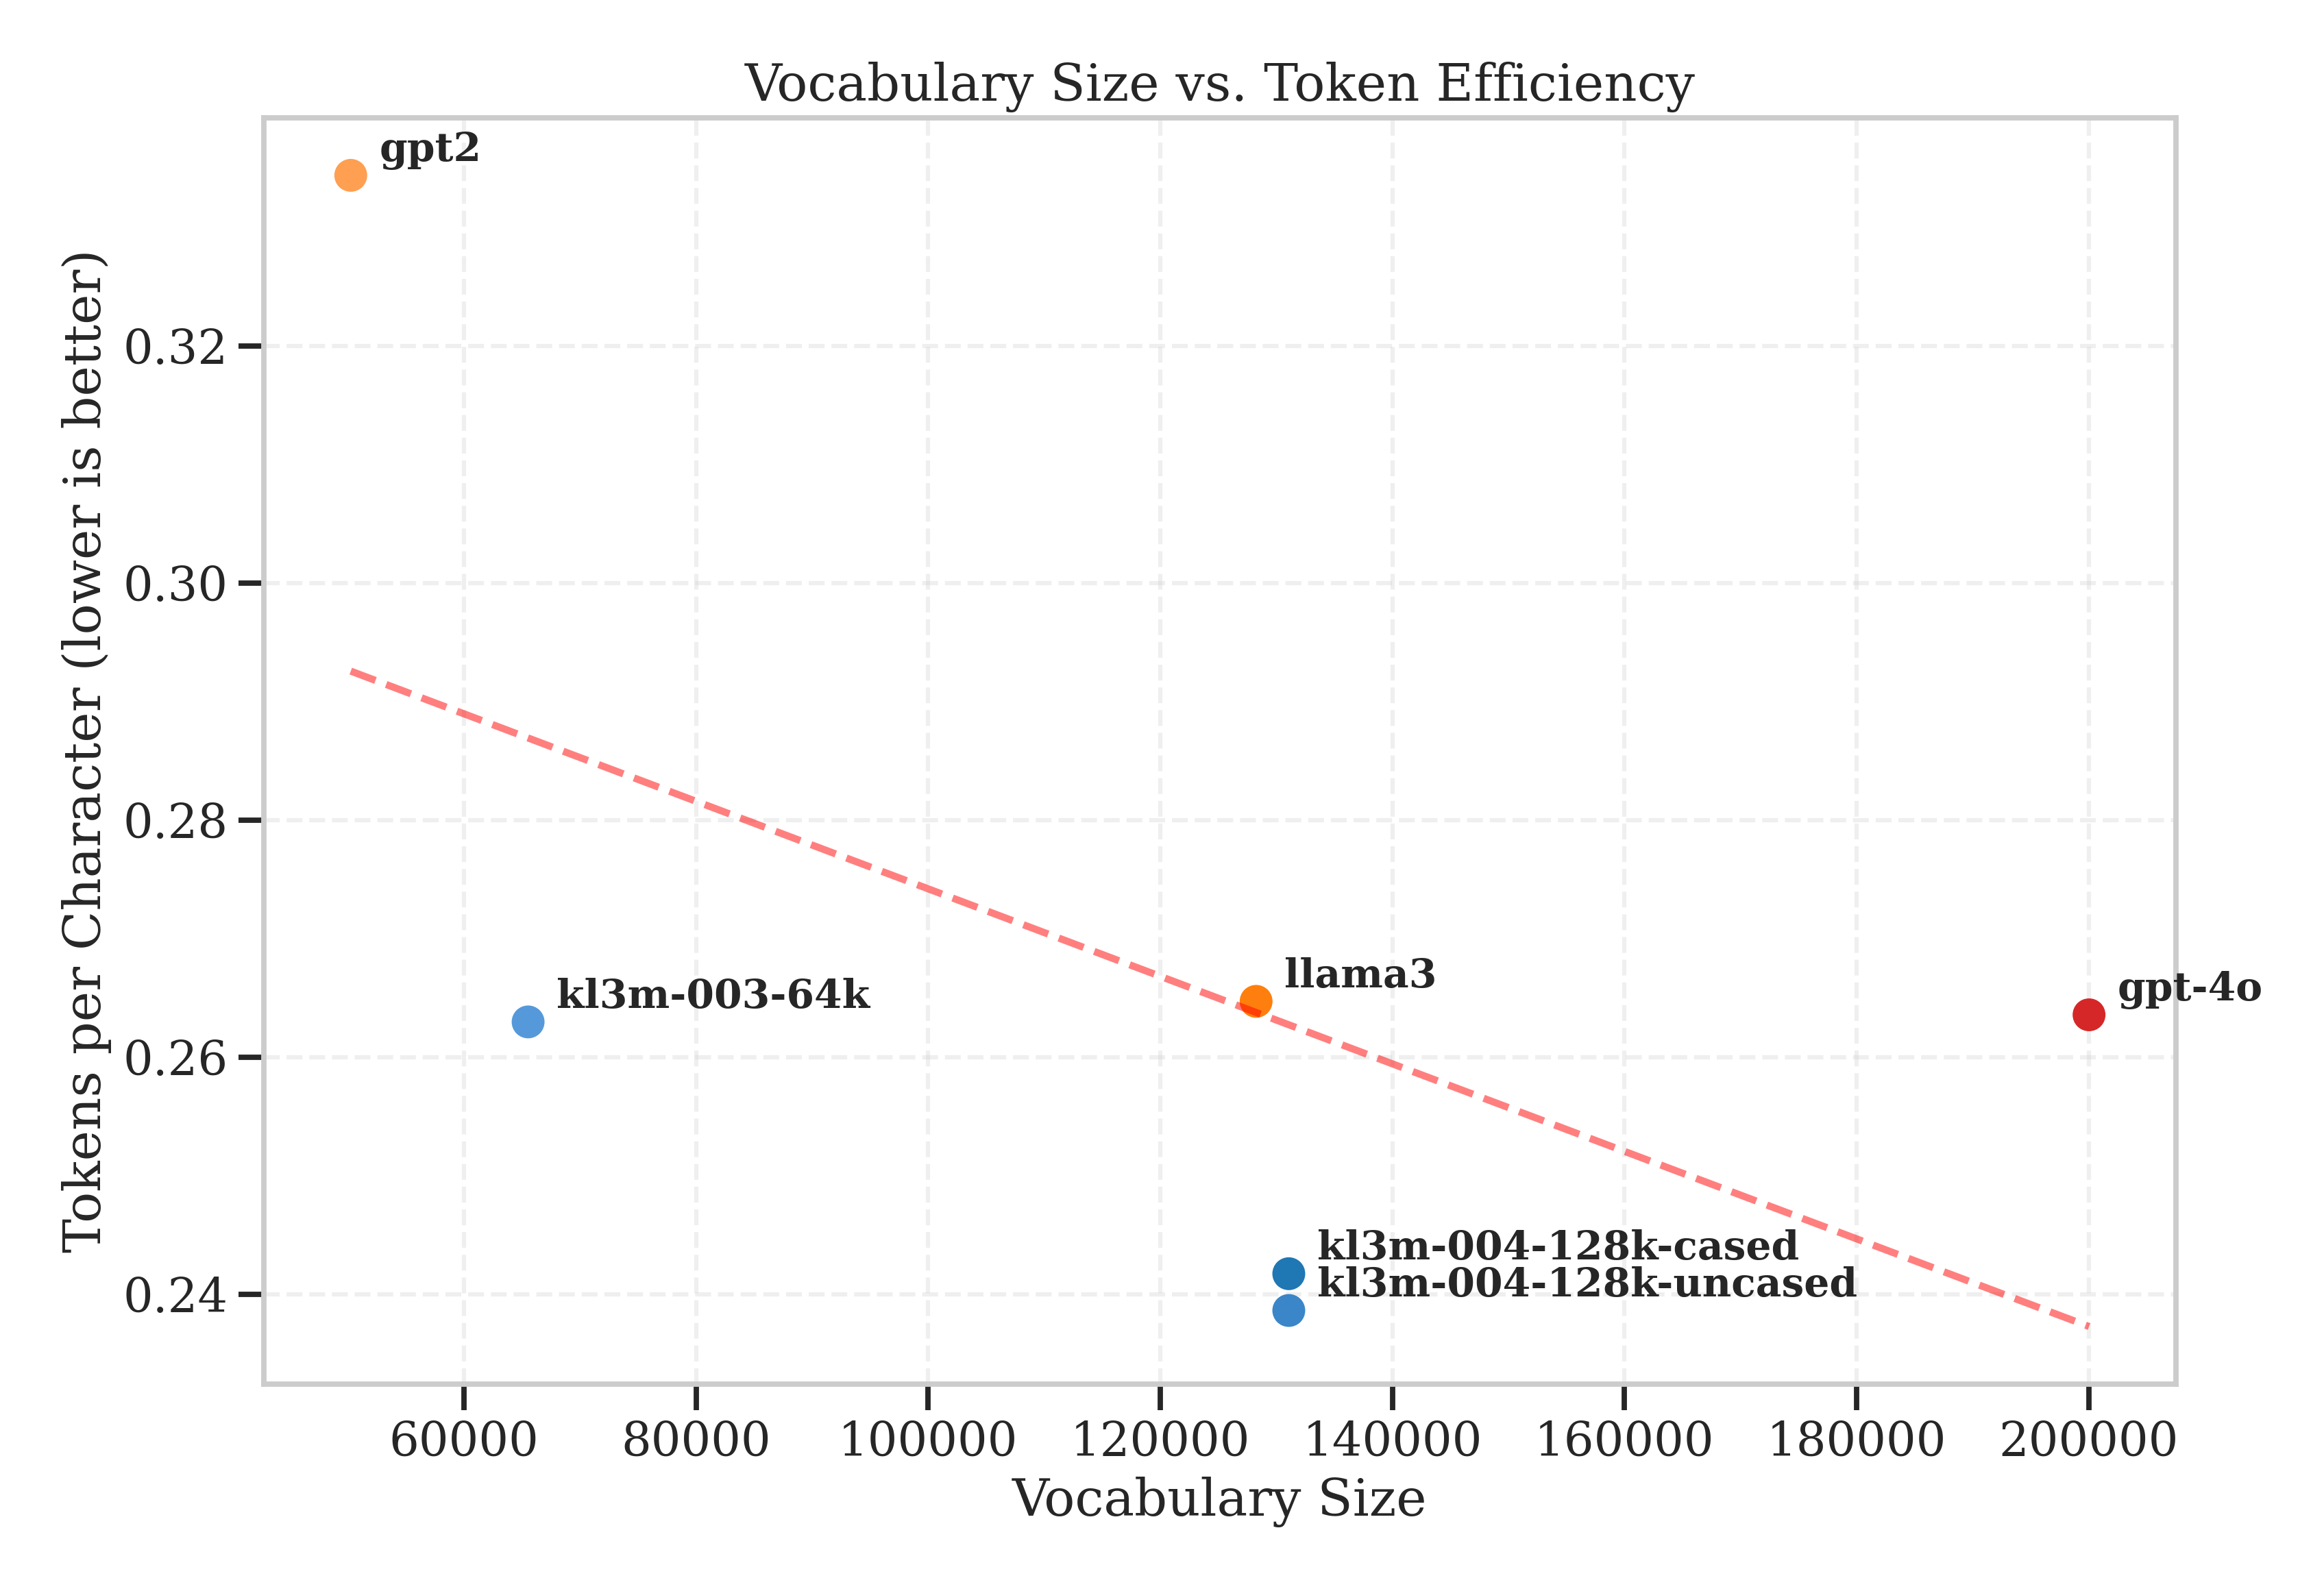
\includegraphics[width=0.85\textwidth]{figures/vocab_size_vs_efficiency.png}
    \caption{Relationship between vocabulary size and tokenization efficiency. KL3M tokenizers achieve superior efficiency despite having comparable vocabulary sizes to other tokenizers.}
    \label{fig:vocab_size_vs_efficiency}
\end{figure*}

\subsection{Domain Term Representation}

Efficient representation of domain-specific terminology directly impacts how accurately and efficiently models can process specialized content. A key advantage of domain-optimized tokenizers is their ability to represent technical terms with fewer tokens, preserving semantic integrity. Tables~\ref{tab:domain-term-comparison} and \ref{tab:domain-term-aggregate} demonstrate how KL3M tokenizers achieve substantial improvements in this critical dimension:

% Domain-specific term tokenization comparison
\begin{table*}[ht]
\centering
\caption{Token count comparison for domain-specific terminology across tokenizers}
\label{tab:domain-term-comparison}
\small
\begin{tabular}{@{}llrrrrrr@{}}
\toprule
Domain & Term & \rotatebox{90}{kl3m\mbox{-}004\mbox{-}128k\mbox{-}cased} & \rotatebox{90}{kl3m\mbox{-}004\mbox{-}128k\mbox{-}uncased} & \rotatebox{90}{gpt\mbox{-}4o} & \rotatebox{90}{llama3} & \rotatebox{90}{roberta\mbox{-}base} & \rotatebox{90}{gpt2} \\
\midrule
Legal & 11 U.S.C. \S 362(a) & \textbf{6} & \textbf{6} & 10 & 11 & 15 & 13 \\
 & res judicata & \textbf{2} & \textbf{2} & 3 & 5 & 6 & 4 \\
 & stare decisis & \textbf{3} & \textbf{3} & 4 & 5 & 7 & 5 \\
 & habeas corpus & \textbf{2} & \textbf{2} & 4 & 5 & 5 & 3 \\
 & certiorari & \textbf{1} & \textbf{1} & 3 & 4 & 5 & 3 \\
 & de novo review & \textbf{3} & \textbf{3} & \textbf{3} & 4 & 6 & 4 \\
 & 28 C.F.R. \S 14.2(a) & \textbf{8} & \textbf{8} & 12 & 13 & 16 & 14 \\
 & 42 U.S.C. \S 1983 & \textbf{5} & \textbf{5} & 9 & 10 & 11 & 9 \\
 & Fed. R. Civ. P. 12(b)(6) & \textbf{10} & \textbf{10} & 14 & 15 & 16 & 14 \\
 & prima facie & \textbf{2} & \textbf{2} & 3 & 5 & 6 & 4 \\
\addlinespace[0.5em]
Financial & EBITDA & \textbf{1} & \textbf{1} & 3 & 4 & 5 & 3 \\
 & P/E ratio & 4 & 4 & \textbf{3} & 4 & 6 & 4 \\
 & 10-K filing & 4 & 4 & \textbf{3} & 4 & 6 & 4 \\
 & SEC Form 8-K & \textbf{5} & \textbf{5} & \textbf{5} & 6 & 7 & \textbf{5} \\
 & quarterly dividend & \textbf{2} & \textbf{2} & 3 & 4 & 5 & 3 \\
 & year-over-year growth & 6 & 6 & \textbf{4} & 5 & 8 & 6 \\
 & Basel III compliance & \textbf{3} & \textbf{3} & 4 & 5 & 6 & 4 \\
 & GAAP accounting & \textbf{2} & \textbf{2} & 3 & 4 & 5 & 3 \\
 & ROI analysis & \textbf{2} & \textbf{2} & \textbf{2} & 3 & 5 & 3 \\
 & market capitalization & \textbf{2} & \textbf{2} & \textbf{2} & 4 & 5 & 3 \\
\bottomrule
\end{tabular}
\end{table*}

% Domain-specific term aggregate statistics
\begin{table*}[ht]
\centering
\caption{Average token count by domain across tokenizers}
\label{tab:domain-term-aggregate}
\begin{tabular}{lrrr}
\toprule
Tokenizer & Legal Terms & Financial Terms & Overall \\
\midrule
kl3m\mbox{-}004\mbox{-}128k\mbox{-}cased & \textbf{4.20} & \textbf{3.10} & \textbf{3.65} \\
kl3m\mbox{-}004\mbox{-}128k\mbox{-}uncased & \textbf{4.20} & \textbf{3.10} & \textbf{3.65} \\
gpt\mbox{-}4o & 6.50 & 3.20 & 4.85 \\
llama3 & 7.70 & 4.30 & 6.00 \\
roberta\mbox{-}base & 9.30 & 5.80 & 7.55 \\
gpt2 & 7.30 & 3.80 & 5.55 \\
\bottomrule
\end{tabular}
\end{table*}

The data reveals significant differences in how tokenizers handle specialized terminology:

\begin{itemize}
    \item \textbf{Legal terminology}: \texttt{kl3m-004-128k-cased} encodes terms like "certiorari" and "habeas corpus" in just 1-2 tokens, while \texttt{gpt-4o} and \texttt{LLaMA3} require 3-5 tokens. For complex legal citations (e.g., "42 U.S.C. § 1983"), our cased tokenizer requires 5 tokens compared to 9-10 tokens for other tokenizers.
    
    \item \textbf{Financial terminology}: Terms like "EBITDA" are represented as a single token in \texttt{kl3m-004-128k-cased} but require 3-5 tokens in other tokenizers. Even for complex terms like "Basel III compliance," our cased tokenizer achieves a 25-40\% reduction in token count.
    
    \item \textbf{Overall efficiency}: As shown in Table~\ref{tab:domain-term-aggregate}, \texttt{kl3m-004-128k-cased} requires an average of just 3.65 tokens for domain-specific terms, compared to 4.85 for \texttt{gpt-4o} (33\% more), 6.00 for \texttt{LLaMA3} (64\% more), and 5.55 for \texttt{gpt-2} (52\% more).
\end{itemize}

This more efficient representation offers two key advantages: (1) it reduces computational overhead by requiring fewer tokens for domain-specific content, and (2) it preserves semantic integrity by keeping domain concepts as atomic units rather than fragmenting them into semantically meaningless subwords. This preservation of semantic boundaries is particularly valuable for fine-tuning models on domain-specific tasks where conceptual precision is critical.

\subsection{Character Tokenizer Performance}

Our specialized KL3M character tokenizers (4K, 8K, and 16K variants) represent a distinct approach optimized for text normalization and error correction. Unlike standard tokenizers, these are designed with deliberately constrained vocabulary sizes and maximum token lengths (2-5 characters), resulting in more consistent tokenization patterns that facilitate character-level transformations.

Comparative analysis across these variants revealed that:
\begin{itemize}
    \item The 4K variant provides maximum granularity for pure character-level operations
    \item The 8K variant offers an optimal balance between granularity and efficiency for general text correction
    \item The 16K variant incorporates larger domain-specific character sequences beneficial for specialized correction tasks
\end{itemize}

This approach is particularly valuable for legal and financial documents where errors from OCR, transcription, or manual entry can significantly alter meaning and where preserving exact formatting is critical.

\subsubsection{Text Error Correction Example}

Table \ref{tab:error_example} demonstrates how the character-level tokenizers process text errors compared to standard tokenizers. Consider the text "Thc Vnited S tates 5enate is nesp0nslbe for the" (an error-containing version of "The United States Senate is responsible for the," representative of OCR mistakes, transcription errors, or user typos). 

\begin{table*}[htbp]
    \centering
    \small
    \caption{Character-level tokenization of text errors from test data}
    \label{tab:error_example}
    \begin{tabular}{p{3.2cm}p{5.5cm}p{5.5cm}p{2.5cm}}
        \toprule
        \textbf{Tokenizer} & \textbf{Error Text} & \textbf{Correct Text} & \textbf{Notes} \\
        & \textit{Thc Vnited S tates 5enate is nesp0nslbe for the} & \textit{The United States Senate is responsible for the} & \\
        \midrule
        kl3m-004-char-4k-cased & 
        ["Th", "c", " V", "n", "it", "ed", " S", " t", "at", "es", " 5", "en", "ate", 
        " is", " n", "esp", "0", "ns", "l", "be", " f", "or", " t", "he"] & 
        ["The", " Un", "it", "ed", " St", "at", "es", " S", "en", "ate", 
        " is", " re", "sp", "ons", "ib", "le", " f", "or", " t", "he"] & 
        Preserves character positioning \\
        \midrule
        kl3m-004-char-8k-cased & 
        ["Th", "c", " V", "nit", "ed", " S", " t", "at", "es", " 5", "en", "ate", 
        " is", " n", "esp", "0", "ns", "l", "be", " f", "or", " t", "he"] & 
        ["The", " Un", "it", "ed", " St", "at", "es", " S", "en", "ate", 
        " is", " re", "sp", "ons", "ib", "le", " f", "or", " t", "he"] & 
        Balances character groups \\
        \midrule
        kl3m-004-char-16k-cased & 
        ["Th", "c", " V", "n", "ited", " S", " t", "ates", " 5", "en", "ate", 
        " is", " n", "esp", "0", "ns", "l", "be", " for", " the"] & 
        ["The", " Un", "ited", " St", "ates", " Sen", "ate", 
        " is", " re", "sp", "ons", "ible", " for", " the"] & 
        Larger character groupings \\
        \midrule
        gpt-4o & 
        ["Th", "c", " V", "n", "ited", " S", " t", "ates", " ", "5", "en", "ate", 
        " is", " n", "esp", "0", "n", "sl", "be", " for", " the"] & 
        ["The", " Un", "ited", " States", " Sen", "ate", 
        " is", " respons", "ible", " for", " the"] & 
        Less consistent boundaries \\
        \bottomrule
    \end{tabular}
\end{table*}

As shown in Table \ref{tab:error_example}, the character-level tokenizers precisely tokenize each character or small character group in the error text. This fine-grained tokenization allows models to:

\begin{itemize}
    \item Make direct character-to-character mappings (e.g., recognizing "Thc" → "The")
    \item Detect and correct transposition errors (e.g., "nesp0nslbe" → "responsible")
    \item Handle insertion/deletion errors (e.g., "S tates" → "States")
    \item Correct character confusions and substitutions (e.g., "5enate" → "Senate", "0" → "o")
\end{itemize}

As Table \ref{tab:error_example} illustrates, the key advantage of KL3M character tokenizers compared to standard BPE approaches is their consistent tokenization patterns between error-containing and correct text forms. While standard tokenizers like \texttt{gpt-4o} produce radically different token boundaries when handling errors, our character tokenizers maintain stable segmentation patterns that enable more effective learning of correction mappings.

This structured approach to character-level tokenization benefits several practical use cases:

\begin{itemize}
    \item \textbf{OCR post-processing}: Correcting scanning errors in legal documents and financial statements where errors can significantly alter meaning
    \item \textbf{Transcription normalization}: Standardizing court transcripts, congressional records, and regulatory filings where formatting consistency is critical
    \item \textbf{Document digitization}: Converting legacy documents where character-level errors are common but systematic
    \item \textbf{Legal citation standardization}: Ensuring consistent formatting of case citations, statutory references, and regulatory citations
\end{itemize}

The efficiency gains from this approach are particularly valuable in large-scale document processing workflows where both accuracy and computational efficiency are critical considerations.